\documentclass[11pt,a4paper]{article}

% Compile with XeLaTeX. The body font is genuine Times New Roman.
\usepackage{fontspec}
\ifdefined\TimesFontPath
  \setmainfont{Times.TTF}[
    Path=\TimesFontPath,
    BoldFont=Timesbd.TTF,
    ItalicFont=Timesi.TTF,
    BoldItalicFont=Timesbi.TTF]
\else
  \setmainfont{Times New Roman}
\fi
\setsansfont{TeX Gyre Heros}
\setmonofont{Latin Modern Mono}[Scale=0.85]
\usepackage[margin=2.5cm]{geometry}
\usepackage{amsmath}
\usepackage{unicode-math}
\setmathfont{TeX Gyre Termes Math}
\usepackage{graphicx}
\usepackage{booktabs,array}
\usepackage{caption,subcaption}
\usepackage{float}
\usepackage[section]{placeins}
\usepackage{needspace}
\usepackage{enumitem}
\usepackage{xcolor}
\usepackage{listings}
\usepackage{microtype}
\usepackage[hidelinks]{hyperref}
\usepackage{bookmark}
\graphicspath{{figures/}}
\setlength{\parskip}{0.35em}
\setlength{\parindent}{0pt}
\setlength{\emergencystretch}{2em}
\captionsetup{font=small,labelfont=bf}
\lstset{language=Python,basicstyle=\ttfamily\footnotesize,
 keywordstyle=\color{blue!60!black}\bfseries,
 commentstyle=\color{green!35!black}\itshape,
 stringstyle=\color{red!50!black},frame=single,
 rulecolor=\color{black!25},breaklines=true,showstringspaces=false,
 columns=fullflexible,keepspaces=true}
\newcommand{\code}[1]{\texttt{#1}}
\makeatletter
\newcommand{\tabledata}[1]{\@@input data/#1.tex }
\makeatother
\newcommand{\studentname}{Md Zunayedul Islam}
\newcommand{\githublink}{https://github.com/zunaaaaayed/AdvTopicsLabs}
% Generated from the saved experiment artifacts.
\newcommand{\NParameters}{4,740,516}
\newcommand{\BaselineVal}{73.61\%}
\newcommand{\BaselineTest}{73.23\%}
\newcommand{\SelectedVal}{72.77\%}
\newcommand{\SelectedTest}{72.97\%}
\newcommand{\SelectedEvalVal}{72.75\%}
\newcommand{\Threshold}{72.61\%}
\newcommand{\SelectedZeros}{2,844,310}
\newcommand{\SelectedNonzero}{1,896,206}
\newcommand{\HistogramThreshold}{0.001140}
\newcommand{\BaselineMB}{19.00}
\newcommand{\MaskedMB}{37.97}
\newcommand{\DenseMB}{19.00}
\newcommand{\FinalMB}{37.97}

\hypersetup{pdftitle={Lab 1: Pruning},
 pdfauthor={Md Zunayedul Islam},pdfsubject={Advanced Topics in IPCVAI, Lab 1}}

\begin{document}
\begin{titlepage}
\centering
\definecolor{coveraccent}{HTML}{243B53}
\vspace*{0.8cm}
{\fontsize{18}{23}\selectfont\bfseries Universit\'e de Bordeaux\par}
\vspace{0.65cm}
{\fontsize{12}{17}\selectfont
Erasmus Mundus Joint Masters in Artificial Intelligence\\
for Image Processing and Computer Vision\par}
\vspace{0.3cm}
{\large 2025--2027\par}

\vspace{2.7cm}
{\color{coveraccent}\rule{0.22\linewidth}{0.8pt}\par}
\vspace{0.65cm}
{\color{coveraccent}\fontsize{34}{41}\selectfont\bfseries Lab 1: Pruning\par}
\vspace{0.55cm}
{\fontsize{15}{21}\selectfont
Advanced Topics in Image Processing\\
and Computer Vision\par}

\vfill
{\small Submitted by\par}
\vspace{0.15cm}
{\fontsize{15}{20}\selectfont\bfseries \studentname\par}
\vspace{0.75cm}
{\small Code and experiments\par}
\vspace{0.12cm}
{\small\expandafter\url\expandafter{\githublink}\par}
\vspace{0.6cm}
{\normalsize 21 October 2026\par}
\vspace*{1cm}
\end{titlepage}
\pagenumbering{roman}
\begingroup
\small
\setlength{\parskip}{0pt}
\tableofcontents
\endgroup
\newpage
\pagenumbering{arabic}

\section{Introduction}

This lab studies how far a trained CIFAR-100 classifier can be pruned while retaining useful classification accuracy. I implemented the baseline and the pruning procedures in the three supplied Python files, preserved the exercise statements, and used a saved train/validation split throughout. My baseline is a VGG-style network with \NParameters{} trainable parameters. Its best checkpoint reaches \BaselineVal{} validation accuracy and \BaselineTest{} test accuracy.

I compared layer-by-layer L1 pruning, global L1 pruning, five epochs of fine-tuning after global pruning, and repeated pruning followed by fine-tuning. The same validation rule was used throughout: \textbf{keep the highest measured sparsity whose accuracy is within one percentage point of the baseline}. The threshold is therefore \Threshold. Model selection did not use the test set.

The main result is that \textbf{global pruning followed by fine-tuning produces a model with 60\% zero parameters and \SelectedTest{} test accuracy}, a loss of only 0.26 percentage points relative to the baseline. In contrast, layerwise pruning at just 20\% sparsity reduces validation accuracy to 7.44\%. Figure~\ref{fig:overview} summarises the measured curves. All results in this report come from my own saved artifacts; the friend's report was used only as a reference for organisation and presentation.

\begin{figure}[htbp]
\centering
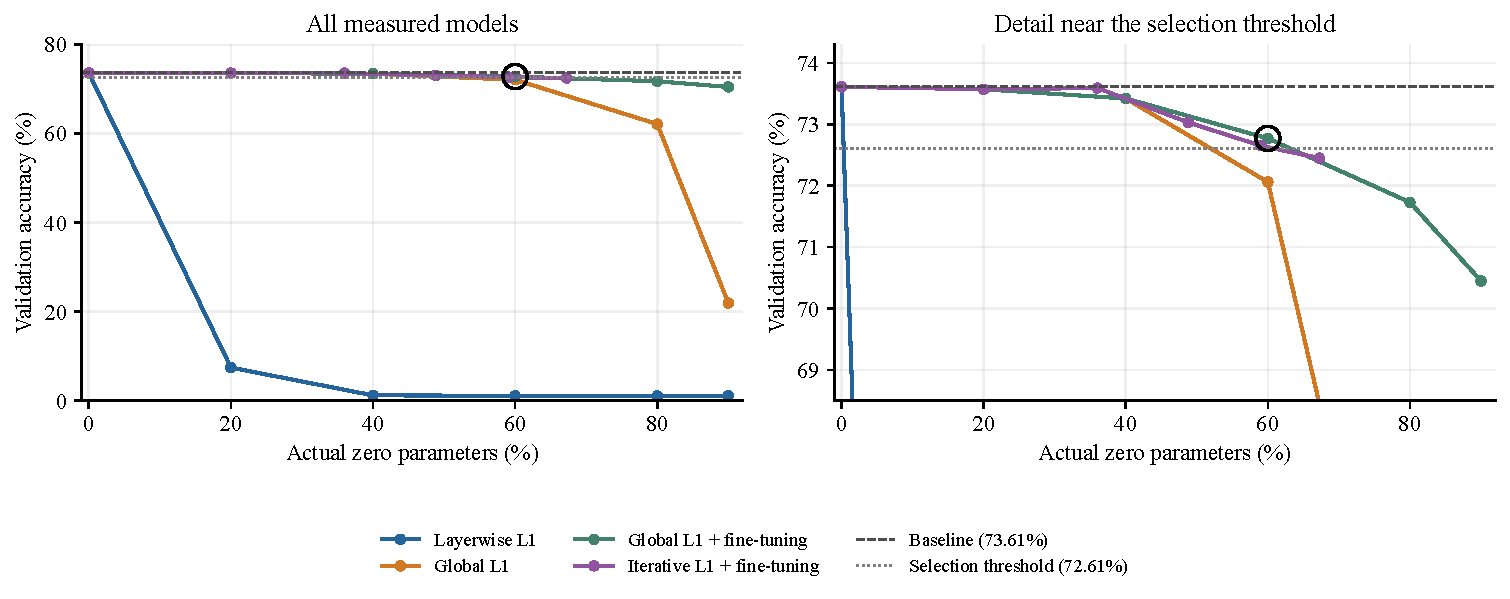
\includegraphics[width=\linewidth]{overview.pdf}
\caption{Validation accuracy against actual sparsity. The right panel enlarges the region near the selection threshold. Markers are measured checkpoints; connecting lines are visual guides, not additional experiments. The circle marks the selected 60\% sparse model.}
\label{fig:overview}
\end{figure}

\section{Background}

\subsection{Granularity, scope and selection criterion}

Magnitude pruning removes connections with small absolute values. In unstructured pruning, each scalar parameter can be selected independently; structured pruning instead removes groups, such as channels. The scope determines whether each tensor is pruned separately or all eligible tensors are ranked together. Magnitude pruning combined with retraining is an established model-reduction procedure~\cite{han2015}.

In my layerwise implementation, every eligible weight and bias tensor receives the same requested pruning fraction. Global pruning applies a single ranking to the union of those tensors. Thus a layer can lose far more or far less than the requested overall fraction. The total sparsity reported here is
\begin{equation}
 s=\frac{\sum_{\theta\in\mathcal P}\#\{i:\theta_i=0\}}
          {\sum_{\theta\in\mathcal P}|\theta|},
\end{equation}
where $\mathcal P$ contains the weights and biases of all convolutional, batch-normalisation and linear layers. Batch-normalisation running statistics are buffers and are excluded. Small rounding differences between requested and measured sparsity are retained in the raw JSON files.

\subsection{Masks, fine-tuning and storage}

PyTorch's pruning utilities~\cite{pytorchpruning} represent an effective parameter as
\begin{equation}
 \theta_{\mathrm{effective}}=\theta_{\mathrm{orig}}\odot M,
 \qquad M_i\in\{0,1\}.
\end{equation}
The original parameter remains trainable, and a mask determines which entries participate in the forward computation. I keep this representation during fine-tuning so masked entries cannot become nonzero in the effective parameter. Checkpoint loading reinstates the pruning representation before loading the state dictionary.

The function \code{prune.remove} materialises the masked values and removes the reparameterisation~\cite{pytorchremove}. This does not shrink tensor dimensions or convert the result into a sparse storage format. Consequently, this report distinguishes \emph{zero parameters}, \emph{nonzero parameters} and \emph{file size}; a high zero fraction alone is not evidence of faster inference or smaller dense checkpoints.

\section{Experimental Setup}

\subsection{Dataset, preprocessing and split}

CIFAR-100 consists of 100 classes of $32\times32$ colour images~\cite{cifar100}. I split the official 50,000 training images into 40,000 training and 10,000 validation images and kept the official 10,000 test images for final evaluation. The split uses seed 42 and is stored in \code{artifacts/baseline/train\_val\_split.pt}. Loading checks the seed, label-order fingerprint, split size, disjointness and coverage. Pruning never generates a replacement split.

Training preprocessing consists of a random crop to $32\times32$ with four pixels of padding, random horizontal flipping, tensor conversion and channel-wise normalisation. The channel means are $(0.5071,0.4867,0.4408)$ and the standard deviations are $(0.2675,0.2565,0.2761)$. Validation and test preprocessing omit augmentation. This is mean/standard-deviation normalisation; the resulting values are not restricted to $[-1,1]$.

\subsection{Selection and comparison protocol}

For the independent sweeps, I tested requested sparsities of 0, 20, 40, 60, 80 and 90\%. Each ratio starts from a freshly constructed network loaded with the same baseline checkpoint. Exercise~4 reloads Exercise~3's masked checkpoints. Exercise~5 intentionally carries one model forward across pruning steps.

For a method with measured candidate set $\mathcal S$, my rule is
\begin{equation}
 s^*=\max\{s\in\mathcal S:\ a_{\mathrm{val}}(s)\geq0.7361-0.01\}.
\end{equation}
The result is the sparsest \emph{tested} eligible model. For example, selecting 60\% does not establish whether an untested 70\% model would satisfy the rule. Each fine-tuning call retains the best validation state among the starting state (epoch 0) and its five additional epochs. It can therefore keep the pre-fine-tuning model when every update reduces validation accuracy.

\subsection{Implementation and environment}

The implementation uses \code{src/model.py}, \code{train.py} and \code{pruning.py}. Shared data loading, evaluation and checkpoint utilities are in the existing model file, so no independent Python evaluation file was added. The \code{--exercise evaluate} option evaluates a saved checkpoint without training.

The recorded training and pruning environment is Python 3.13.5, PyTorch 2.14.1+cu130, torchvision 0.29.1+cu130 and CUDA 13.0 on an NVIDIA RTX 4000 Ada Generation. Other recorded versions are NumPy 2.2.4, torchmetrics 1.9.0, Pillow 12.3.0 and Matplotlib 3.10.1. Seed 42, zero data-loader workers and deterministic PyTorch algorithms are used. Configurations include source-code and artifact hashes. This makes the run auditable, but does not guarantee identical floating-point results across different hardware and software.

\section{Exercise 0: Building a Baseline}

\subsection{Architecture}

I used a small VGG-style network, inspired by the repeated $3\times3$ convolutions of VGG~\cite{vgg}. There are four blocks, each with two convolution--batch-normalisation--ReLU sequences. The channel widths are 64, 128, 256 and 512. A $2\times2$ max-pooling layer follows each of the first three blocks, giving spatial resolutions $32\rightarrow16\rightarrow8\rightarrow4$. There is no fourth max-pooling layer. Global average pooling reduces the final feature maps to one value per channel, and a linear layer produces 100 logits.

\begin{table}[htbp]
\centering
\small
\caption{Architecture and trainable parameter distribution. Spatial sizes are after each block, including its pooling when present. Convolutional biases are included.}
\label{tab:architecture}
\begin{tabular}{llrrr}
\toprule
Stage & Operations & Channels & Output & Parameters \\
\midrule
\tabledata{architecture_rows}
\midrule
Total & & & & \NParameters \\
\bottomrule
\end{tabular}
\end{table}

The last block contains approximately 74.72\% of all trainable parameters. This uneven distribution helps explain why a single global threshold can remove many connections from the late convolutions while preserving most parameters in smaller layers. The complete model has 17 parameterised layers: eight convolutions, eight batch-normalisation layers and one classifier. Each contributes a weight and a bias tensor, giving 34 tensors to prune.

\subsection{Optimisation and SSH recovery}

I used cross-entropy loss and SGD with initial learning rate 0.1, momentum 0.9, weight decay $5\times10^{-4}$ and batch size 128. The planned schedule contains 200 epochs with cosine learning-rate decay. The checkpoint with the highest validation accuracy is kept for all later experiments.

The original training process stopped after epoch 65 following an SSH disconnect. At that point only the best weights, split, configuration and history had been saved; the best weights corresponded to epoch 54 with 58.15\% validation accuracy. Recovery verified those weights against the saved validation result, restarted at epoch 55, and restored the cosine schedule's position. \textbf{Optimizer momentum and random-number states had not been saved and were reset.} The final retained history therefore combines the original epochs 1--54 with the recovered epochs 55--200; it is not an uninterrupted 200-epoch experiment.

This event is recorded in \code{recovery.json}, and the original history through epoch 65 remains in the backup directory. The updated training code saves a full checkpoint atomically after each completed epoch, including optimizer, scheduler and random states. Later execution was detached with \code{tmux} to survive a lost SSH terminal.

\subsection{Results and interpretation}

\begin{figure}[htbp]
\centering
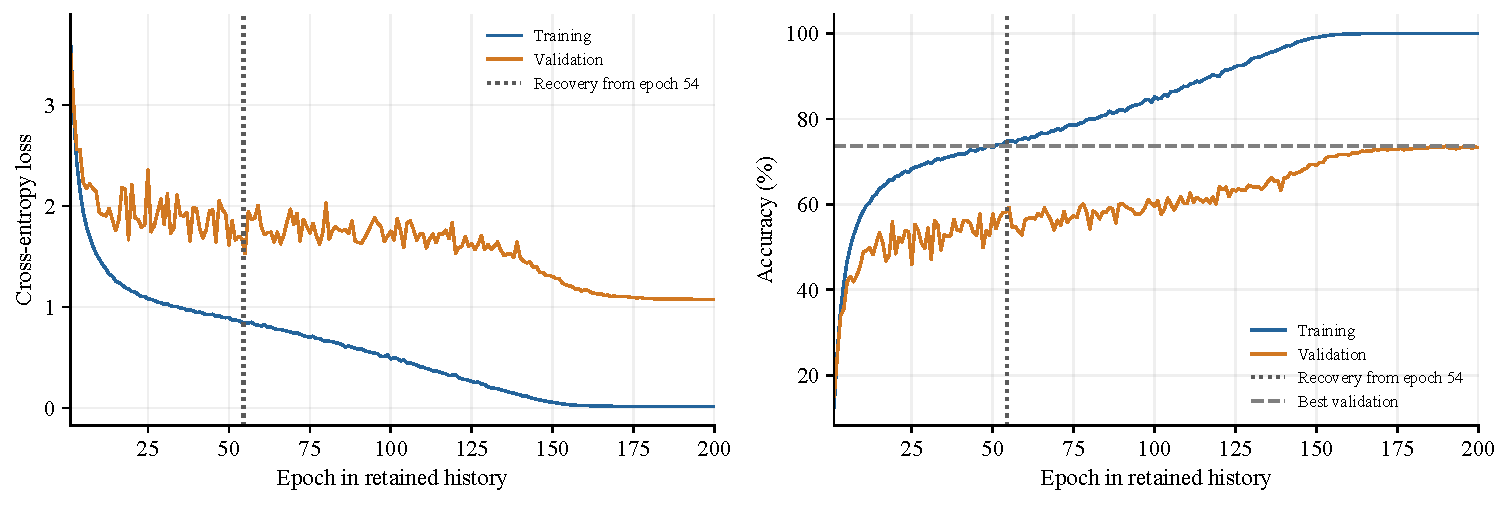
\includegraphics[width=\linewidth]{baseline_training.pdf}
\caption{Retained baseline history: training/validation loss and accuracy. The vertical line marks recovery after epoch 54. Discarded original epochs 55--65 are preserved separately and are not spliced into the recovered trajectory.}
\label{fig:baseline}
\end{figure}

The best checkpoint is epoch 190: validation accuracy is \BaselineVal{} and final test accuracy is \BaselineTest. This exceeds the approximately 65--70\% target mentioned in the instructions. At epoch 200, training accuracy is 99.985\%, while validation accuracy is 73.33\%. The large training--validation gap indicates substantial overfitting, even though the model generalises well enough for the pruning experiments.

The training loss falls from 3.7088 at epoch 1 to 0.0137 at epoch 200. Validation accuracy continues to improve late in the schedule: it is 59.62\% at epoch 100, 69.13\% at epoch 150 and reaches 73.61\% at epoch 190. The final-epoch model is therefore not the one used as the baseline. The validation and test accuracies of the selected baseline differ by 0.38 percentage points; this is descriptive evidence, not a formal generalisation guarantee.

\section{Exercise 1: Pruning a Pre-trained Model}

\subsection{Implementation}

I collected the 34 weight/bias tensors and called \code{prune.l1\_unstructured} independently on each with \code{amount=0.2}. This includes batch-normalisation scales and offsets, as requested by the instruction to prune layer weights and biases. Mask buffers identify which entries survive. I then called \code{prune.remove} on each pruned parameter and saved the resulting ordinary state dictionary.

\begin{figure}[htbp]
\centering
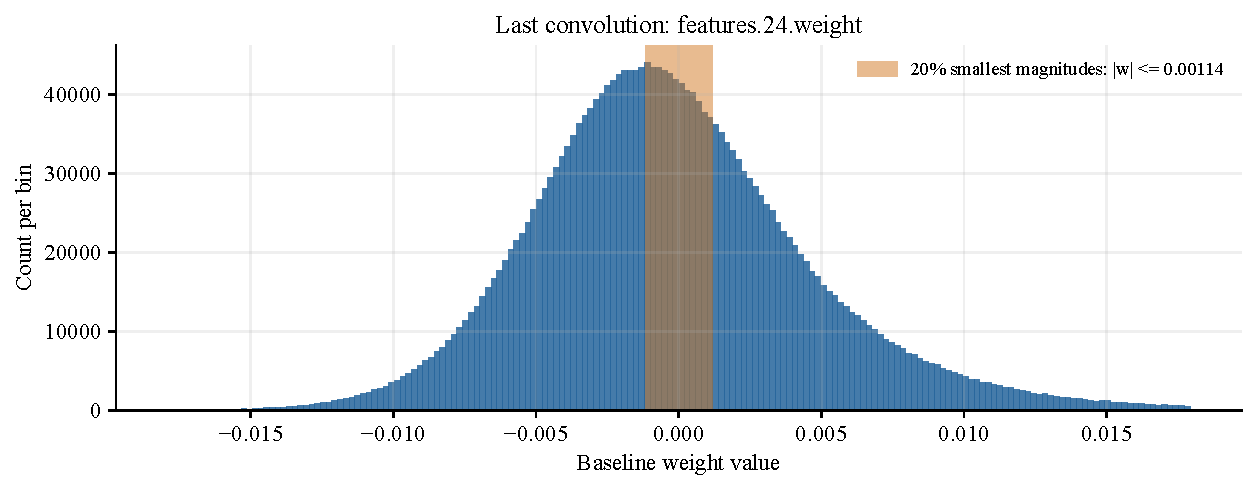
\includegraphics[width=0.86\linewidth]{weight_histogram.pdf}
\caption{Baseline weights in the last convolution, \code{features.24.weight}. The shaded interval contains the 20\% smallest absolute weights in this tensor; its magnitude threshold is approximately \HistogramThreshold. The histogram display is limited to the central 99.5\% magnitude range for readability; selection uses all entries.}
\label{fig:histogram}
\end{figure}

\subsection{Results and discussion}

At approximately 20\% overall sparsity, validation accuracy falls from 73.61\% to \textbf{7.44\%}, a loss of 66.17 percentage points. Validation cross-entropy rises from 1.0785 to 5.4269. The saved model has the intended zero fraction, so the relevant conclusion is that this uniform per-tensor policy is highly damaging for this trained architecture.

A plausible explanation is that the same fraction is removed from both very large convolutional tensors and small, potentially sensitive tensors. In particular, a batch-normalisation scale acts on a whole output channel; zeroing it changes that channel's input-dependent contribution. The offset can still be nonzero, so a zero scale should not automatically be described as deleting the entire channel. I did not run an ablation that leaves batch normalisation unpruned, so this explanation remains a hypothesis.

The baseline dense state dictionary occupies approximately \BaselineMB{} MB. A masked global checkpoint occupies about \MaskedMB{} MB, while its ordinary dense export occupies \DenseMB{} MB (decimal MB, $10^6$ bytes). These measured sizes illustrate the storage effect of retaining masks. Removing the reparameterisation returns dense storage to approximately the baseline size; it does not produce a file proportional to the number of surviving connections.

\section{Exercise 2: Accuracy / Sparsity Ratio Curve}

\subsection{Measured curve}

For each requested sparsity I reloaded the baseline, repeated layerwise L1 pruning, removed the masks and evaluated on the saved validation split. The results were saved immediately after each measurement. Figure~\ref{fig:layerwise} is the original experiment plot.

\begin{figure}[htbp]
\centering
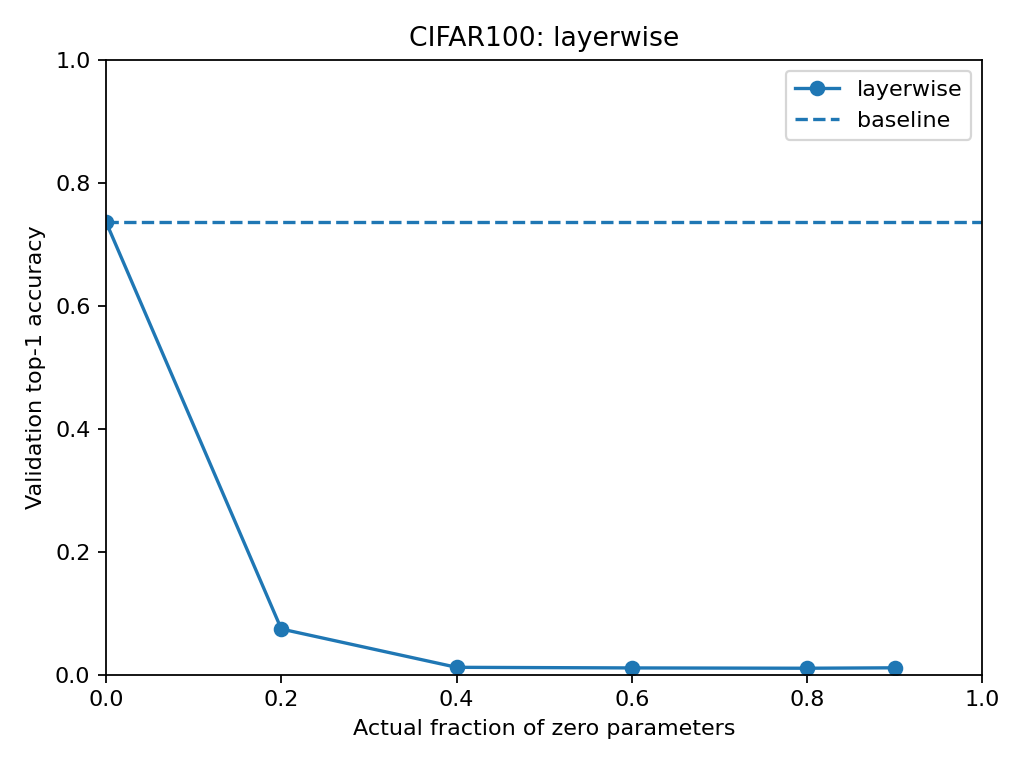
\includegraphics[width=0.72\linewidth]{layerwise_curve.png}
\caption{Exercise~2: the original saved layerwise pruning curve. Sparsity and accuracy axes are fractions; Table~\ref{tab:layerwise} expresses them as percentages.}
\label{fig:layerwise}
\end{figure}

\begin{table}[htbp]
\centering
\caption{Layerwise L1 pruning without fine-tuning. Accuracy drops are absolute percentage points relative to the baseline.}
\label{tab:layerwise}
\begin{tabular}{rrrr}
\toprule
Actual sparsity & Validation accuracy & Validation loss & Accuracy drop (pp) \\
\midrule
\tabledata{layerwise_rows}
\bottomrule
\end{tabular}
\end{table}

\subsection{Comments and model choice}

The 20\% point reproduces Exercise~1 exactly. Accuracy is already close to the 1\% chance level by 40\% sparsity and stays around that level through 90\%. Several losses exceed $\log(100)\approx4.605$, the cross-entropy of a uniform prediction over 100 classes. This shows that the resulting probabilities can be badly calibrated as well as inaccurate.

Under the \Threshold{} threshold, \textbf{the only eligible measured model is the unpruned model}. I therefore keep 0\% sparsity for this method. The experiment contains no points between 0 and 20\%, so it does not establish whether a smaller nonzero fraction would be acceptable. A finer low-sparsity sweep and a batch-normalisation ablation would be useful follow-up experiments, but neither is reported as completed here.

\section{Exercise 3: Global Pruning}

\subsection{Implementation and results}

I passed the same 34 parameter tuples to \code{prune.global\_unstructured}, using \code{prune.L1Unstructured} and each requested ratio~\cite{pytorchglobal}. Each candidate starts from the baseline. I saved the masked checkpoints for fine-tuning and exported ordinary dense state dictionaries separately.

\begin{figure}[htbp]
\centering
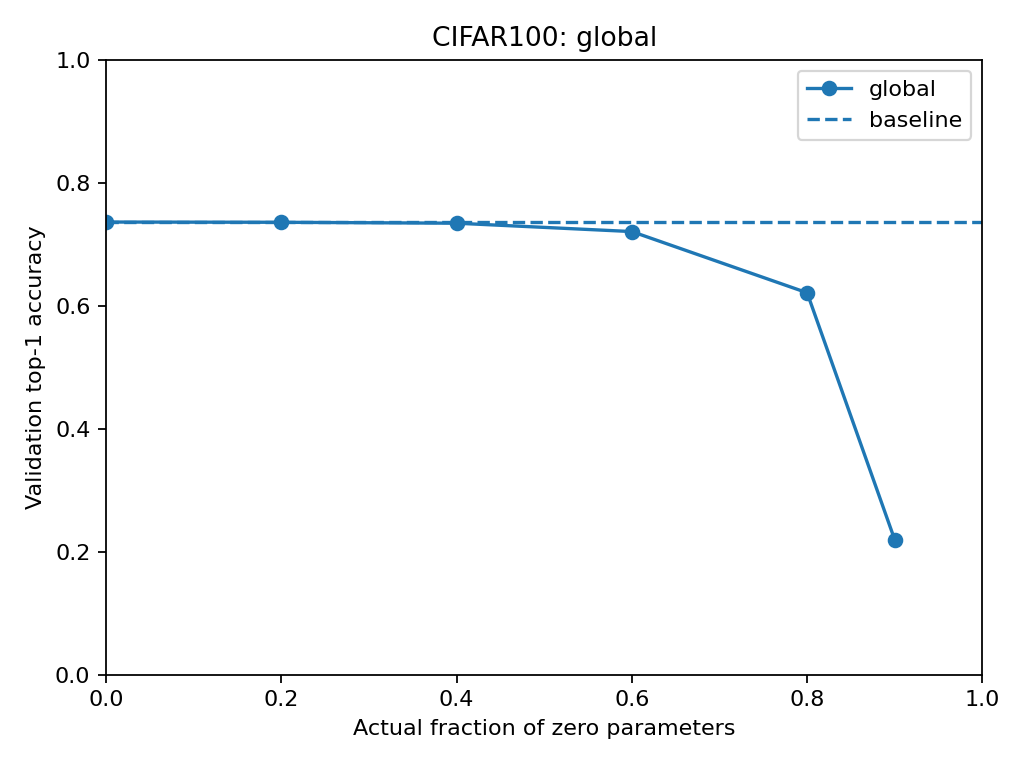
\includegraphics[width=0.72\linewidth]{global_curve.png}
\caption{Exercise~3: original saved global-pruning curve. The contrast with Figure~\ref{fig:layerwise} shows the effect of changing the ranking scope while keeping the magnitude criterion.}
\label{fig:global}
\end{figure}

\begin{table}[htbp]
\centering
\caption{Layerwise versus global pruning on the same validation split, without fine-tuning.}
\label{tab:global}
\begin{tabular}{rrrr}
\toprule
Actual sparsity & Layerwise accuracy & Global accuracy & Global drop (pp) \\
\midrule
\tabledata{global_rows}
\bottomrule
\end{tabular}
\end{table}

Global pruning preserves accuracy much better: at 20\% it retains 73.57\%, compared with 7.44\% for layerwise pruning. At 40\%, accuracy remains 73.42\%, only 0.19 percentage points below baseline. The 60\% point is 72.06\%, below the threshold. The selected global model is therefore \textbf{40\% sparse at 73.42\% validation accuracy}. Its zero count is 1,896,206, leaving 2,844,310 nonzero trainable parameters.

\subsection{Where the zeros are placed}

\begin{figure}[htbp]
\centering
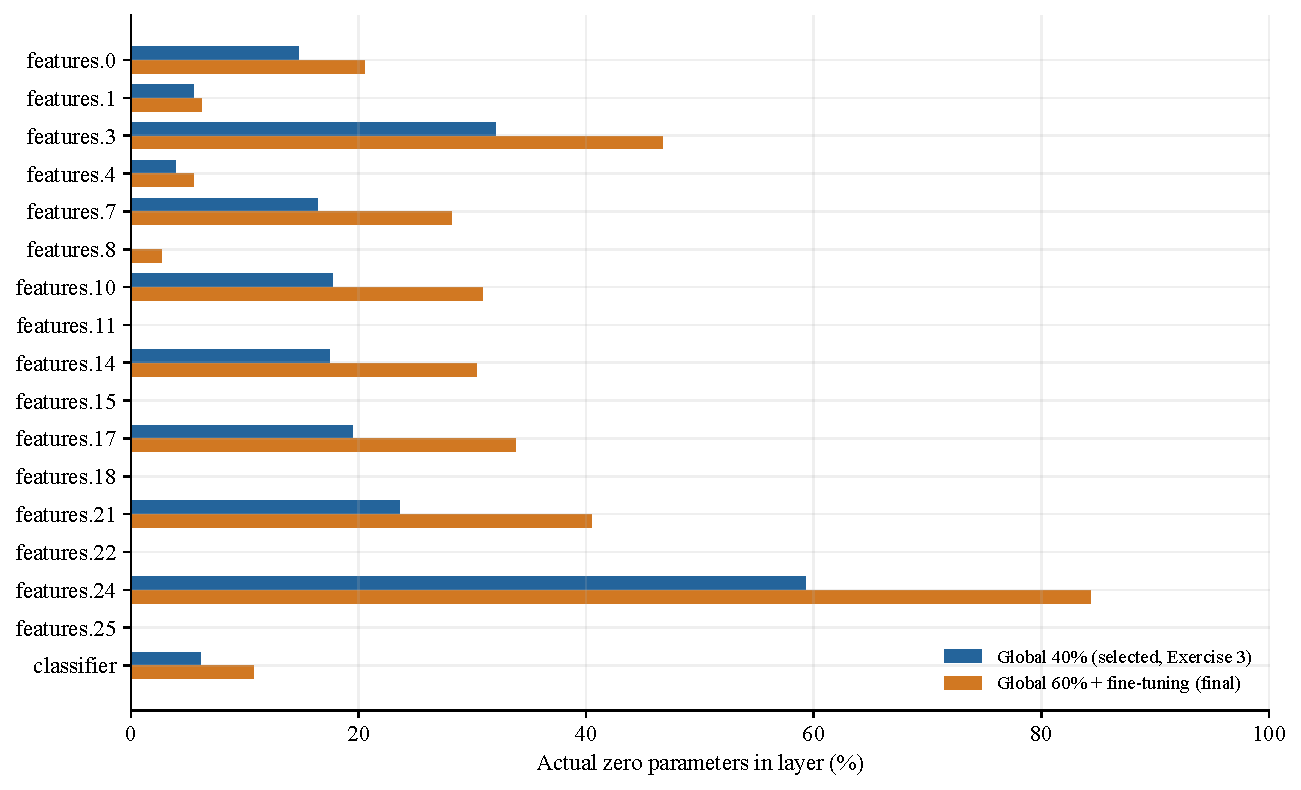
\includegraphics[width=0.96\linewidth]{layer_sparsity.pdf}
\caption{Per-layer sparsity of the selected global 40\% model and the final 60\% sparse fine-tuned model. Weight and bias entries are counted together. Numerical values appear in Table~\ref{tab:layer-sparsities}.}
\label{fig:layers}
\end{figure}

At 40\% overall sparsity, the last convolution has 59.26\% zero entries, whereas the first convolution has 14.73\% and the classifier has 6.15\%. Most batch-normalisation layers remain entirely nonzero. This supports the interpretation that a uniform per-tensor quota removes relatively important entries from small tensors, while a global quota can concentrate many zeros in large late convolutions. Nevertheless, magnitude scales differ between layer types; the observed success of global pruning does not establish that cross-layer magnitude is an ideal universal importance measure.

\begin{table}[htbp]
\centering
\small
\caption{Numerical sparsity of every parameterised layer, rounded to two decimal places. The Global 40\% column answers Exercise~3 for its selected model; the Final 60\% column provides the comparison with the fine-tuned model selected in Exercise~4. Counts include weights and biases, but exclude running statistics. Values come from the saved per-layer JSON files.}
\label{tab:layer-sparsities}
\begin{tabular}{llrrr}
\toprule
Layer & Type & Parameters & Global 40\% & Final 60\% \\
\midrule
\tabledata{layer_rows}
\midrule
Overall & & \NParameters & 40.00\% & 60.00\% \\
\bottomrule
\end{tabular}
\end{table}

\section{Exercise 4: Re-training a Pruned Model}

\subsection{Protocol and checkpoint selection}

Each globally pruned checkpoint was fine-tuned for five epochs at initial learning rate 0.01, with SGD momentum 0.9, weight decay $5\times10^{-4}$ and a five-epoch cosine schedule. The training data and saved split were unchanged, and masks remained active. I retained the best validation state among epochs 0--5.

The zero-sparsity candidate acts as a control for the extra optimisation. This control is important because the baseline had already converged at a much lower learning rate than 0.01. Restarting with that rate can temporarily worsen validation accuracy even without pruning.

\begin{figure}[htbp]
\centering
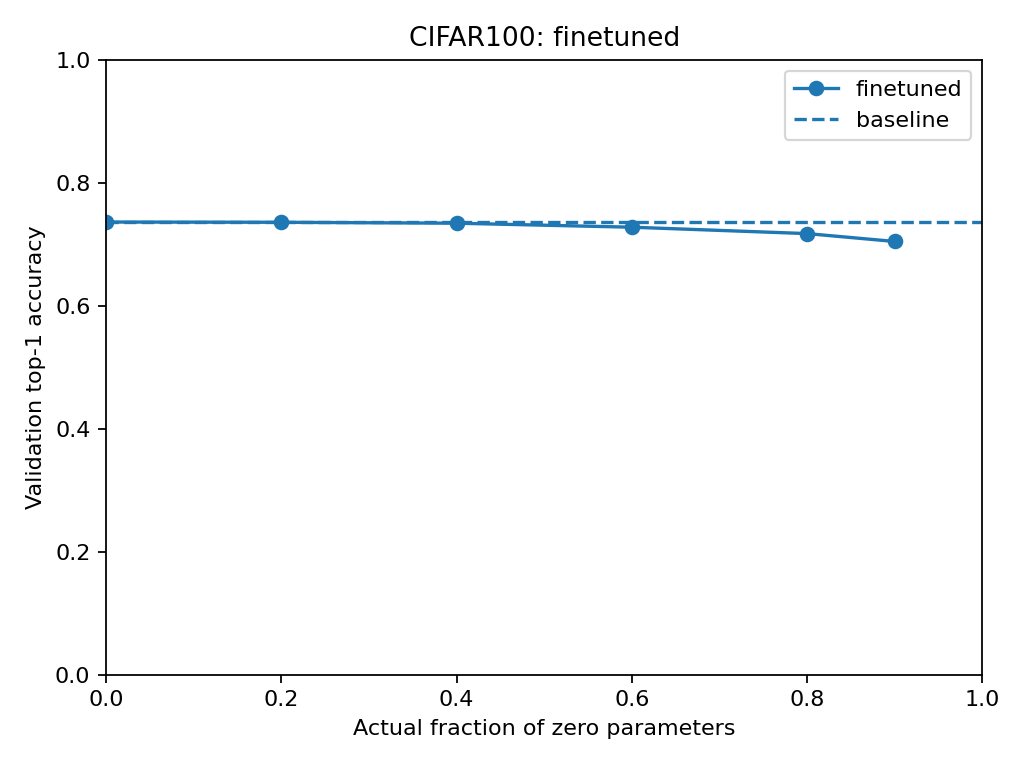
\includegraphics[width=0.72\linewidth]{finetuned_curve.png}
\caption{Exercise~4: original saved curve of retained checkpoints after fine-tuning. At low sparsity the best retained state can be the starting state rather than any updated epoch.}
\label{fig:finetuned}
\end{figure}

\begin{table}[htbp]
\centering
\small
\caption{Validation accuracy before fine-tuning, at the final extra epoch, and in the retained checkpoint. Gain compares the retained state with the state before fine-tuning.}
\label{tab:finetuned}
\begin{tabular}{rrrrr}
\toprule
Sparsity & Before & Epoch 5 & Retained best & Gain (pp) \\
\midrule
\tabledata{finetuned_rows}
\bottomrule
\end{tabular}
\end{table}

\subsection{Comments on the curve}

\begin{figure}[htbp]
\centering
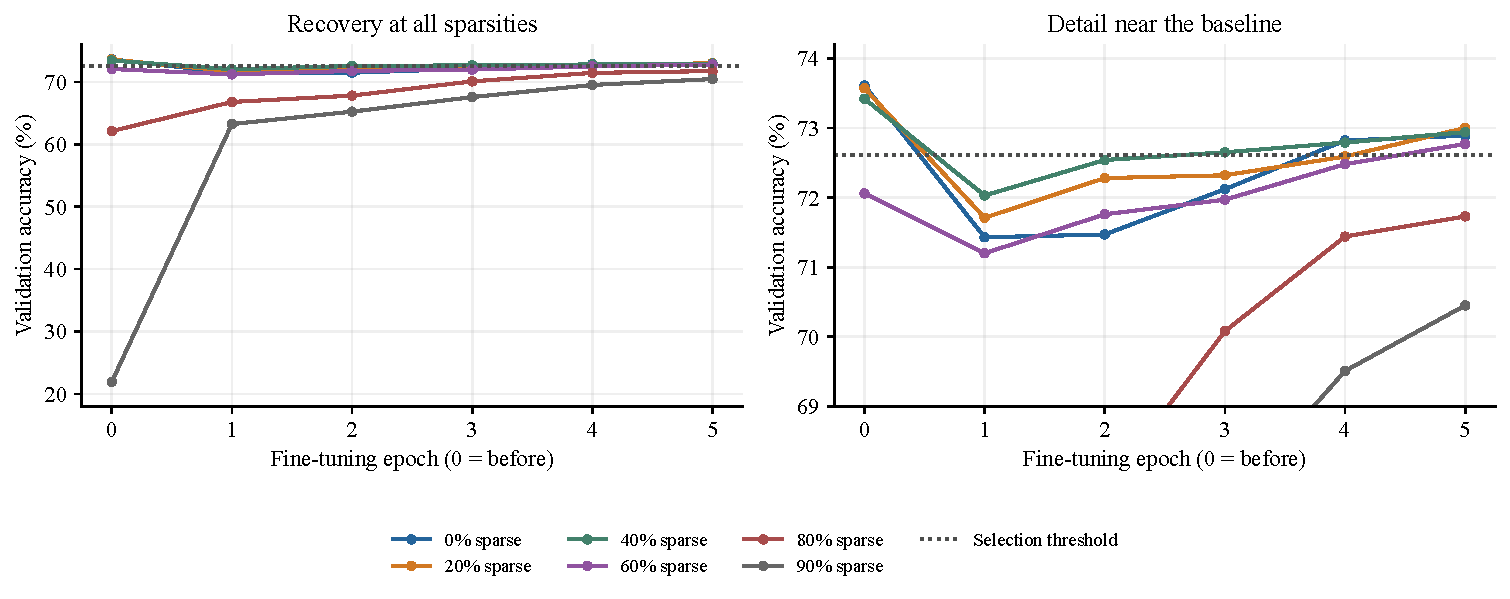
\includegraphics[width=\linewidth]{finetuning_history.pdf}
\caption{Measured validation histories for each sparsity. Epoch 0 is the globally pruned model before fine-tuning. The right panel shows low-sparsity degradation and high-sparsity recovery near the selection threshold.}
\label{fig:finetuninghistory}
\end{figure}

Fine-tuning is especially helpful after aggressive pruning. At 80\% sparsity, accuracy rises from 62.11\% to 71.73\%, a gain of 9.62 percentage points. At 90\%, it rises from 21.93\% to 70.45\%, a gain of 48.52 points. These results show that the surviving connections can recover much of the classifier's performance, although both candidates remain below the one-point threshold.

At 0, 20 and 40\% sparsity, no updated epoch outperforms the starting state. The retained values are therefore identical to Exercise~3. For the control, the first extra epoch drops to 71.43\% and epoch 5 recovers to 72.89\%, still below the original 73.61\%. It would be misleading to describe the retained control accuracy as an improvement caused by five more epochs: the checkpoint policy kept epoch 0.

\subsection{Which model would I keep?}

The \textbf{60\% sparse model reaches \SelectedVal{} validation accuracy}, a drop of 0.84 percentage points, and satisfies the \Threshold{} threshold. It contains \SelectedZeros{} zeros and \SelectedNonzero{} nonzero trainable parameters. The 80\% candidate misses the rule by 0.88 percentage points. I therefore select \code{finetuned\_0.6.pt} among the measured candidates. Fine-tuning increases the selected sparsity from 40\% to 60\%, although it does not establish an optimum between these tested ratios.

\section{Exercise 5: Iterative Training and Pruning}

\subsection{Cumulative schedule}

For this exercise I loaded the baseline once, then performed five rounds on the same cumulative model. Each round prunes 20\% of the currently unmasked entries globally and runs the five-epoch fine-tuning procedure. Ignoring integer rounding, the cumulative requested sparsity after step $t$ is
\begin{equation}
 s_t=1-(1-0.2)^t=1-0.8^t.
\end{equation}
The resulting sequence is 20, 36, 48.8, 59.04 and 67.232\%, rather than the independent sweep's 20, 40, 60, 80 and 90\%. Each round starts a new fine-tuning optimiser and schedule; masks and effective model state accumulate across rounds.

\begin{figure}[htbp]
\centering
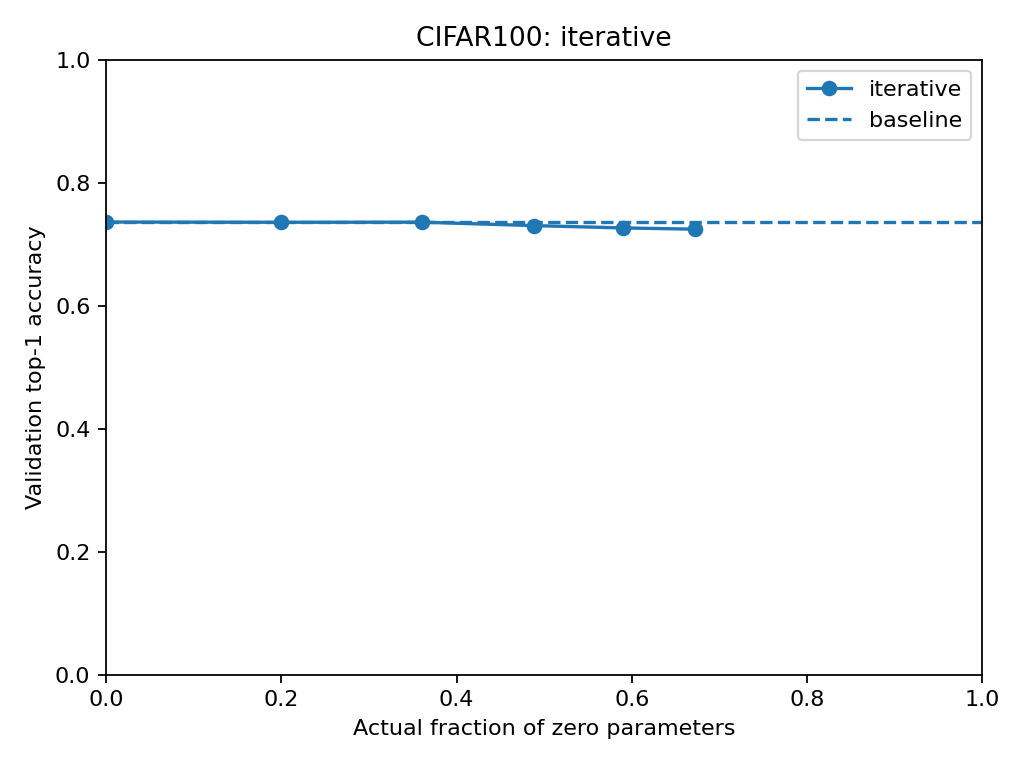
\includegraphics[width=0.72\linewidth]{iterative_curve.png}
\caption{Exercise~5: the original saved iterative curve, including the unpruned starting point and five cumulative pruning steps.}
\label{fig:iterative}
\end{figure}

\begin{table}[htbp]
\centering
\caption{Iterative retained checkpoints. The epoch count is the number of extra epochs executed up to that step, not necessarily the age of every retained update, since a round can keep its starting state.}
\label{tab:iterative}
\begin{tabular}{rrrrr}
\toprule
Step & Actual sparsity & Extra epochs run & Validation accuracy & Drop (pp) \\
\midrule
\tabledata{iterative_rows}
\bottomrule
\end{tabular}
\end{table}

\subsection{Comments and model choice}

\begin{figure}[htbp]
\centering
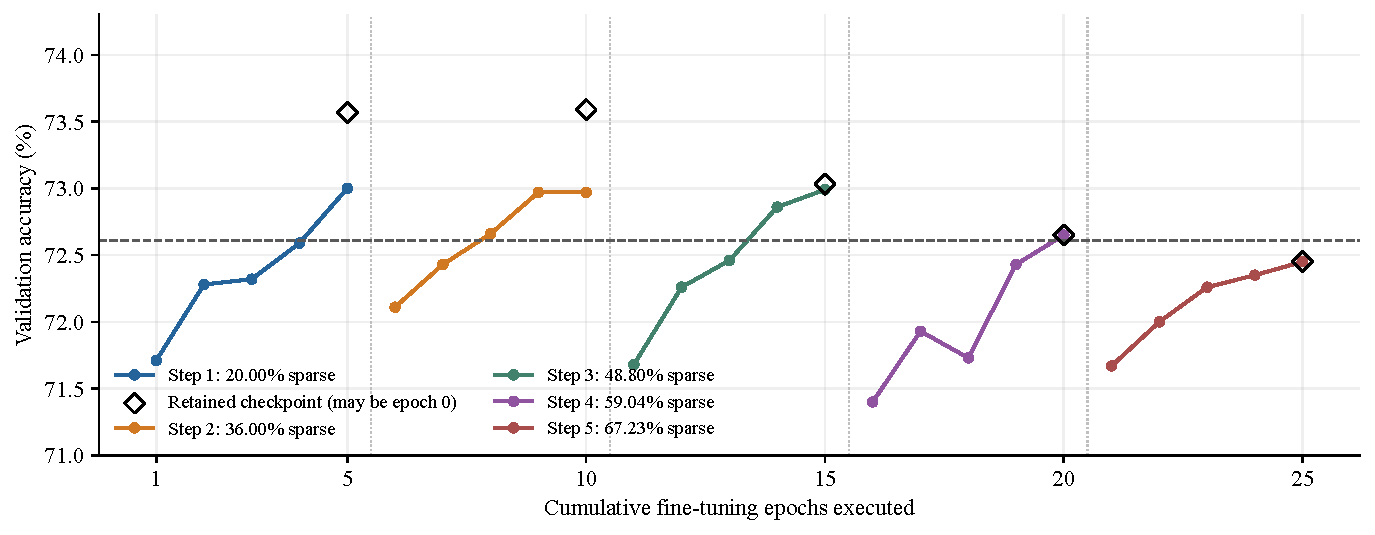
\includegraphics[width=0.98\linewidth]{iterative_history.pdf}
\caption{Within-round validation accuracy during the 25 extra epochs. Lines connect measured epochs within each round only. Diamonds show the retained checkpoint accuracy, which can exceed every updated epoch because the state before fine-tuning is also eligible. The individual pre-fine-tuning evaluations were not saved as a complete separate series.}
\label{fig:iterativehistory}
\end{figure}

The first step retains 73.57\%, exactly matching global pruning at 20\%; the second reaches 73.59\% at 36\% sparsity. Accuracy then declines as sparsity accumulates. Step 4 retains 72.65\% at 59.04\% sparsity, just 0.04 percentage points above the threshold. Step 5 reaches 67.232\% sparsity but has 72.45\% accuracy, below the rule. I therefore keep \textbf{step 4: 59.04\% sparse, 72.65\% validation accuracy}.

The selected one-shot fine-tuned model is slightly sparser (60\%) and has slightly higher validation accuracy (72.77\%) than this selected iterative checkpoint. It also requires only five additional epochs for that candidate, versus 20 executed along the iterative path. These observations favour the one-shot candidate under the tested configuration, but \textbf{they are not a matched-sparsity or matched-training-budget comparison}. Iterative steps were not tested at exactly 60, 80 or 90\%, so no conclusion about iterative superiority at those ratios is supported by these measurements.

Training accuracy during the final iterative round is almost 100\%, while validation remains near 72\%. This is consistent with the baseline's strong training--validation gap. Whether additional regularisation, fewer fine-tuning epochs or a different pruning schedule would improve iterative pruning requires further experiments.

\section{Final Evaluation on the Test Set}

Once the 60\% sparse model was selected using validation accuracy, I ran the existing evaluation command and saved its output to \code{artifacts/pruning/final\_evaluation.log}. Only the baseline and this selected pruned model have reported test measurements.

\begin{table}[htbp]
\centering
\caption{Final test comparison. The validation column used for selecting the pruned model is the saved original experiment result. The separate evaluation returned 72.75\% validation accuracy for that same checkpoint.}
\label{tab:final}
\begin{tabular}{lrrrr}
\toprule
Model & Sparsity & Nonzero parameters & Selection val. & Test accuracy \\
\midrule
Baseline, epoch 190 & 0\% & \NParameters & \BaselineVal & \BaselineTest \\
Global + fine-tuning & 60\% & \SelectedNonzero & \SelectedVal & \textbf{\SelectedTest} \\
\bottomrule
\end{tabular}
\end{table}

\begin{figure}[htbp]
\centering
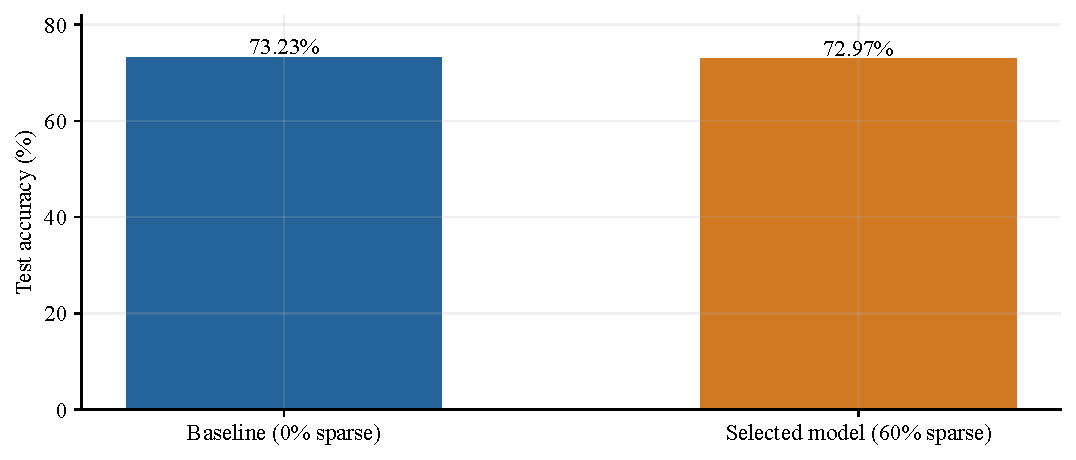
\includegraphics[width=0.78\linewidth]{final_test.pdf}
\caption{Test accuracy of the baseline and the selected pruned checkpoint. These are single-run measurements; no error bars or repeated-seed comparison are available.}
\label{fig:final}
\end{figure}

The selected model reaches \SelectedTest{} test accuracy with test cross-entropy 1.0645. The baseline reaches \BaselineTest{} with loss 1.0619. The difference is \textbf{0.26 percentage points}, corresponding to 26 fewer correct predictions in aggregate over 10,000 images. This is a difference of counts, not a claim that only 26 individual predictions changed between models.

The separate final evaluation reports \SelectedEvalVal{} validation accuracy, whereas the original GPU pruning run saved \SelectedVal. I retain both values rather than silently substituting one for the other. The final evaluation log did not record its device and environment; small numerical differences are a possible explanation, but the saved record does not establish the cause. Both values satisfy the original threshold, and no model was reselected using the test result.

\section{Bonus: Custom Structured Column Pruning}

The bonus implementation inherits from \code{prune.BasePruningMethod}. For a convolutional tensor of shape $(C_{\mathrm{out}},C_{\mathrm{in}},k_h,k_w)$, I interpret a column as an input-channel slice, dimension 1. Its score is
\begin{equation}
 q_c=\sum_{o,u,v}|W_{o,c,u,v}M_{o,c,u,v}|.
\end{equation}
The requested number or fraction of lowest-scoring active columns is masked out across all output channels and spatial positions. The method clones the existing mask, preserves previous zeros and leaves tensors with at most two dimensions unchanged. The existing placeholder docstring is retained, but the effective pruning type is structured.

Synthetic checks verified column ranking, repeated application and previous-mask preservation. \textbf{No full CIFAR-100 bonus run was performed}, so this report gives no structured-pruning accuracy, selected structured model or speed-up. Input-column masking also does not physically remove channels: coordinated architecture changes and explicit profiling would be needed to claim a smaller or faster dense network. This interpretation follows the assignment's wording about columns and differs from output-filter pruning in the reference report.

\section{Overall Discussion}

\begin{table}[htbp]
\centering
\small
\caption{Highest measured sparsity accepted by the one-point rule. Test results are reported only when evaluation actually took place.}
\label{tab:summary}
\begin{tabular}{lrrrl}
\toprule
Method & Sparsity & Val. accuracy & Test accuracy & Extra training \\
\midrule
Baseline & 0\% & 73.61\% & 73.23\% & -- \\
Layerwise L1 & 0\% & 73.61\% & -- & None \\
Global L1 & 40\% & 73.42\% & -- & None \\
Global L1 + fine-tuning & \textbf{60\%} & \textbf{72.77\%} & \textbf{72.97\%} & 5 epochs \\
Iterative global L1 & 59.04\% & 72.65\% & -- & 20 epochs run \\
\bottomrule
\end{tabular}
\end{table}

The strongest contrast is between two uses of the same L1 criterion: a per-tensor 20\% quota loses 66.17 validation points, whereas global 20\% pruning loses only 0.04 points. The layer-sparsity measurements show that the global rule allocates zeros unevenly, especially to the last large convolution. Fine-tuning is useful at high sparsity, but the zero-sparsity control shows that extra optimisation can also harm a converged checkpoint. Including epoch 0 in checkpoint selection prevents that harm from being hidden by an arbitrary final-epoch choice.

There are several limits to these conclusions. All experiments use one seed and one baseline, and the baseline includes a documented weights-only recovery. The sparsity grid is coarse, and the iterative and independent schedules use different target ratios and budgets. Only one fine-tuning setting was tested. The explanation involving batch-normalisation sensitivity was not isolated by ablation. The sparse model still has dense tensor shapes, and its masked file is approximately \FinalMB{} MB; neither inference latency nor sparse-format storage was benchmarked. A 60\% zero fraction should therefore not be advertised as a measured 60\% reduction in memory or runtime.

\Needspace{11\baselineskip}
\section{Conclusion}

I trained and pruned a \NParameters-parameter VGG-style CIFAR-100 classifier using the supplied lab structure. The baseline reached \BaselineTest{} test accuracy. Uniform layerwise pruning was destructive, while global L1 pruning preserved \textbf{73.42\% validation accuracy at 40\% sparsity without retraining}. Five epochs of masked fine-tuning increased the selected measured sparsity to \textbf{60\%}, with \SelectedVal{} validation accuracy and \SelectedTest{} test accuracy.

For this experiment, the final choice is \code{finetuned\_0.6.pt}: \SelectedZeros{} zero parameters, \SelectedNonzero{} nonzero parameters and a test-accuracy drop of 0.26 percentage points. Iterative pruning did not provide a better selected trade-off under the tested schedule. The practical lessons are to preserve the split and baseline, distinguish ranking scope from ranking criterion, account for checkpoint selection during retraining, and separate numerical sparsity from demonstrated compression or acceleration.

\begin{thebibliography}{9}
\raggedright
\bibitem{han2015}
S. Han, J. Pool, J. Tran and W. J. Dally.
\newblock Learning both weights and connections for efficient neural networks.
\newblock \emph{Advances in Neural Information Processing Systems}, 2015.
\newblock \url{https://arxiv.org/abs/1506.02626}.
\bibitem{vgg}
K. Simonyan and A. Zisserman.
\newblock Very deep convolutional networks for large-scale image recognition.
\newblock \emph{International Conference on Learning Representations}, 2015.
\newblock \url{https://arxiv.org/abs/1409.1556}.
\bibitem{cifar100}
A. Krizhevsky, V. Nair and G. Hinton.
\newblock The CIFAR-10 and CIFAR-100 datasets.
\newblock \url{https://www.cs.toronto.edu/~kriz/cifar.html}.
\bibitem{pytorchpruning}
PyTorch contributors. Pruning tutorial.
\newblock \url{https://docs.pytorch.org/tutorials/intermediate/pruning_tutorial.html}.
\bibitem{pytorchremove}
PyTorch contributors. \code{torch.nn.utils.prune.remove}.
\newblock \url{https://docs.pytorch.org/docs/2.14/generated/torch.nn.utils.prune.remove.html}.
\bibitem{pytorchglobal}
PyTorch contributors. \code{torch.nn.utils.prune.global\_unstructured}.
\newblock \url{https://docs.pytorch.org/docs/2.14/generated/torch.nn.utils.prune.global_unstructured.html}.
\end{thebibliography}

\end{document}
